%%%%%%%%%%%%%%%%%%%%%%%%%%%%%%%%%%%%%%%%%
% Short Three-Column Newsletter
% LaTeX Template
% Version 1.0 (11/9/13)
%
% Original author:
% Frits Wenneker (http://www.howtotex.com) 
% With extensive modifications by:
% Vel (vel@latextemplates.com)
% 
% This template has been downloaded from:
% http://www.LaTeXTemplates.com
%
% License:
% CC BY-NC-SA 3.0 (http://creativecommons.org/licenses/by-nc-sa/3.0/)
%
%%%%%%%%%%%%%%%%%%%%%%%%%%%%%%%%%%%%%%%%%

%----------------------------------------------------------------------------------------
%	PACKAGES AND DOCUMENT CONFIGURATIONS
%----------------------------------------------------------------------------------------

\documentclass[10pt,a4paper]{article} % Paper type (a4paper, usletter or legal) and font size (10, 11 or 12)

\setlength\topmargin{-48pt} % Top margin
\setlength\headheight{0pt} % Header height
\setlength\textwidth{7.0in} % Text width
\setlength\textheight{9.5in} % Text height
\setlength\oddsidemargin{-30pt} % Left margin
\setlength\evensidemargin{-30pt} % Left margin (even pages) - only relevant with 'twoside' article option

\usepackage{charter} % Charter font for main content

\frenchspacing % Reduces space after periods to make text more compact for a three-column layout

\usepackage[svgnames]{xcolor} % Enabling colors by their 'svgnames'
\usepackage{graphicx} % Required for including images
\usepackage{amssymb,amsmath} % Math packages
\usepackage{multicol} % Required for the three-column layout of the document
\usepackage{url} % Clickable links
\usepackage{enumitem} % Reduces the amount of space within and between lists with [noitemsep,nolistsep]
\usepackage{marvosym} % Required for the use of symbols
\usepackage{wrapfig} % Allows wrapping text around figures
\usepackage[T1]{fontenc} % Use 8-bit encoding that has 256 glyphs
\usepackage[utf8]{inputenc} % Required for inputting international characters
\usepackage{datetime} % Required for defining a custom date style
\newdateformat{mydate}{\monthname[\THEMONTH] \THEYEAR}
% Set a custom date format
\usepackage[pdfpagemode=FullScreen, colorlinks=false]{hyperref}
% Link colors and PDF behavior in Acrobat
\usepackage{fancyhdr} % Required to define custom headers/footers
\pagestyle{fancy} % Enables the custom headers/footers for all pages following this

\usepackage{geometry} % Required for adjusting page dimensions

\geometry{
	top=1cm, % Top margin
	bottom=1.5cm, % Bottom margin
	left=2cm, % Left margin
	right=2cm, % Right margin
	includehead, % Include space for a header
	includefoot, % Include space for a footer
	%showframe, % Uncomment to show how the type block is set on the page
}


%-----------------------------------------------------------
% Header and footer
\lfoot{\footnotesize % Left footer containing newsletter contact information
    Newsletter title and/or description \\
    \Mundus\ \href{http://www.LaTeXTemplates.com}{LaTeXTemplates.com} \quad
    \Telefon\ (000) 111-1111 \quad
    \Letter\ \href{mailto:email@email.com}{email@email.com}
}

\cfoot{} % Empty center footer

\rfoot{\footnotesize ~\\ Page \thepage} % Right footer - page counter

\renewcommand{\headrulewidth}{0.0pt} % No horizontal rule for the header
\renewcommand{\footrulewidth}{0.4pt} % Horizontal rule separating the footer from the document
%-----------------------------------------------------------

%-----------------------------------------------------------
% Define separators
% \newcommand{\HorRule}[1]{\noindent\rule{\linewidth}{#1}}
\newcommand{\HorRule}{\color{DarkGoldenrod}\rule{\linewidth}{1pt}} % Defines the gold horizontal rule around the title
% Creates a horizontal rule
\newcommand{\SepRule}{\noindent % Creates a shorter separator rule
    \begin{center}
        \rule{250pt}{1pt} % Page width and rule width
    \end{center}
}
%-----------------------------------------------------------

%-----------------------------------------------------------
% Define title and article styles
\newcommand{\NewsletterName}[1]{ % Newsletter title
    \begin{center}
        \Huge \usefont{T1}{fvs}{b}{n} % Use the Bera Sans Bold font
        #1
    \end{center}
    \par \normalsize \normalfont}

\newcommand{\JournalIssue}[1]{ % Date and issue number at the top of the newsletter
    \hfill \textsc{\mydate \today, No #1} % Right-aligned date and issue number
    \par \normalsize \normalfont}

\newcommand{\NewsItem}[1]{ % News item title
    \usefont{T1}{fvs}{n}{n} % Use the Bera Sans Normal font
    \vspace{24pt}\large #1\vspace{3pt} % Print the title with space around it in a larger font size
    \par \normalsize \normalfont}

\newcommand{\NewsAuthor}[1]{ % Author name under the item title
    \hfill by \textsc{#1} \vspace{20pt} % Right-aligned author name in small caps with space after it
    \par \normalfont}


%----------------------------------------------------------------------------------------
%	TITLE SECTION
%----------------------------------------------------------------------------------------

\newcommand{\authorstyle}[1]{{\large\usefont{OT1}{phv}{b}{n}\color{DarkRed}#1}} % Authors style (Helvetica)

\newcommand{\institution}[1]{{\footnotesize\usefont{OT1}{phv}{m}{sl}\color{Black}#1}} % Institutions style (Helvetica)

\usepackage{titling} % Allows custom title configuration


\pretitle{
    \JournalIssue{4} % Issue number
	\vspace{-30pt} % Move the entire title section up
	\HorRule\vspace{10pt} % Horizontal rule before the title
	\fontsize{32}{36}\usefont{OT1}{phv}{b}{n}\selectfont % Helvetica
	\color{DarkRed} % Text colour for the title and author(s)
}

\posttitle{\par\vskip 15pt} % Whitespace under the title

\preauthor{} % Anything that will appear before \author is printed

\postauthor{ % Anything that will appear after \author is printed
	\vspace{10pt} % Space before the rule
	\par\HorRule % Horizontal rule after the title
	\vspace{20pt} % Space after the title section
}

\title{How Quantum Technology will Improve your Life Soon}
% The article title

\author{
	\authorstyle{Sebastian Kock\textsuperscript{1,2,3} and Bonnie
		MacFarlane\textsuperscript{2,3}} % Authors
	\newline\newline % Space before institutions
	\textsuperscript{1}\institution{Universidad Nacional Autónoma de
		México, Mexico City, Mexico}\\ % Institution 1
}
\date{}

\begin{document}

% \NewsletterName{Newsletter Title} % Newsletter title
\maketitle

% \noindent\HorRule{3pt} \\[-0.75\baselineskip] % Thick horizontal rule
% \HorRule{1pt} % Thin horizontal rule

%----------------------------------------------------------------------------------------
%	MAIN NEWS ITEM
%----------------------------------------------------------------------------------------

% \vspace{0.5cm}
% \SepRule
% \vspace{-0.5cm}

\begin{center}
    \begin{minipage}[h]{0.75\linewidth}
        \begin{wrapfigure}{l}{0.41\textwidth}
            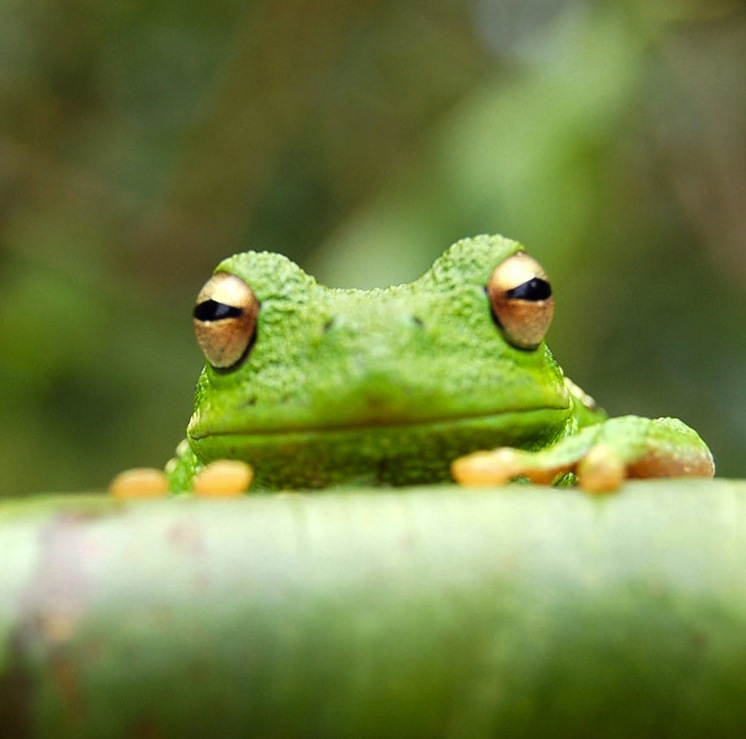
\includegraphics[width=0.42\textwidth]{frog.jpg}
            \\
        \end{wrapfigure}

        \NewsItem{This is the main news item} % Main next item title
        \vspace{3pt} % Some extra whitespace since there is no author as for the news in the body of the newsletter
        \textit{
            Lorem ipsum dolor sit amet, consectetur adipiscing elit. Praesent quis magna
            quis metus gravida tristique. Cras ornare, mauris eu aliquet volutpat, diam
            risus auctor velit, eget molestie odio augue convallis est. Morbi facilisis dui
            quis molestie fringilla. In sed turpis tristique, ornare elit nec, ultrices
            dui. Aliquam porttitor tellus quis dolor laoreet, vitae facilisis est cursus.
            Morbi in risus non mi ornare aliquam nec at lacus. In lobortis velit justo, ut
            malesuada elit interdum facilisis. Nullam venenatis tincidunt suscipit. Nam ut
            gravida est, aliquet sodales lacus.\\ \\
            Integer ut convallis turpis, ut facilisis nunc. Sed pellentesque sapien orci,
            at adipiscing ante laoreet a. Suspendisse sollicitudin, nisl non adipiscing
            volutpat, turpis arcu molestie risus, at blandit diam massa non ante. Quisque a
            massa non quam egestas tincidunt. Aenean lacinia nisi velit, eget tempus ante
            iaculis quis. Nulla et quam in quam malesuada eleifend. Vivamus nec blandit
            orci, iaculis eleifend est.\\ \\
            Pellentesque habitant morbi tristique senectus et netus et malesuada fames ac
            turpis egestas. In hac habitasse platea dictumst. Cras tempor tincidunt
            laoreet. Sed eu luctus ligula. Nam ultricies vulputate semper. Donec et
            ultricies risus. Phasellus vulputate nulla eu nunc fermentum, in viverra justo
            vestibulum. Sed sodales sapien a sapien ullamcorper laoreet. Mauris sodales
            urna dictum velit scelerisque consequat. Aenean ut mauris nec enim posuere
            condimentum at eget lacus.
        }
        \par\hfill --- John Smith
    \end{minipage}
\end{center}

\vspace{0.5cm}
\SepRule % Small horizontal rule after the main news item
\vspace{0.5cm}

%\setlength{\columnsep}{16pt} % Uncomment to manually change the white space between columns
\begin{multicols}{3} % Begin the three-column layout

    %----------------------------------------------------------------------------------------
    %	OTHER NEWS
    %----------------------------------------------------------------------------------------

    \NewsItem{The first news item}
    \NewsAuthor{Author Name}

    Lorem ipsum dolor sit amet, consectetur adipiscing elit. Proin porttitor dui
    non risus fringilla, id elementum quam laoreet. Fusce ac pulvinar mi.
    Pellentesque sapien odio, vulputate eu mi nec, feugiat sagittis velit. Quisque
    ac nulla nec velit imperdiet imperdiet posuere eu odio. Maecenas vitae accumsan
    felis, et porttitor purus. Aliquam erat volutpat. Aenean leo magna, rutrum eget
    est eget, malesuada euismod nisi. Mauris hendrerit nec eros sed posuere.
    Praesent nisi dolor, convallis at nisi mollis, placerat mattis turpis. Donec
    elit ante, suscipit sit amet ante et, sollicitudin faucibus tortor. Suspendisse
    ut mauris ut sem facilisis accumsan. Vestibulum vitae risus nibh.

    Sed lorem justo, tincidunt nec vehicula et, adipiscing vitae mauris.
    Pellentesque rhoncus accumsan urna, et facilisis ipsum vehicula a. Nunc
    pellentesque quis augue in condimentum. Ut vestibulum nunc vel eros aliquam,
    quis venenatis magna commodo. Nam egestas turpis neque, at pretium ipsum
    condimentum sit amet. Etiam eu urna facilisis, ultrices purus ac, fermentum
    orci. Aenean ac ultricies odio. Aenean accumsan urna ut sapien commodo, in
    pulvinar elit tempor. Aliquam dapibus iaculis dui. Suspendisse ut mauris ut sem
    facilisis accumsan. Vestibulum vitae risus nibh. Cras at justo diam. Vestibulum
    ultricies varius ligula vel tincidunt. Duis quis orci consequat elit dictum
    auctor. Suspendisse feugiat quam non justo elementum, eget accumsan leo
    egestas. Aenean dignissim iaculis lorem, vitae rhoncus massa blandit quis.
    Integer dui tellus, cursus eu nisi a, sagittis ultricies massa. Quisque
    pharetra, leo vel vestibulum tincidunt, dolor turpis bibendum sapien, sed
    vestibulum diam augue vel felis. In quis urna tortor. Vestibulum eleifend
    tortor vitae risus suscipit hendrerit. Vestibulum sed ornare lorem. Nam non
    tristique metus. Suspendisse commodo diam a purus ultricies fringilla. Quisque
    rutrum, elit vitae faucibus ultrices, risus lacus condimentum sapien, fringilla
    adipiscing tellus quam sit amet arcu. Vivamus sed orci quis lectus pellentesque
    accumsan.

    %-----------------------------------------------------------

    \NewsItem{The second news item}
    \NewsAuthor{Author Name}

    Donec non nisl a arcu consequat varius. Sed suscipit cursus luctus. Nulla sit
    amet elit augue. Curabitur scelerisque mollis dolor, quis blandit lorem
    condimentum at. Pellentesque sed nibh vel dolor sagittis semper. Maecenas lacus
    enim, suscipit ut suscipit eget, feugiat vitae elit. Sed volutpat justo nisi,
    ac bibendum ante. Sed lacinia eros in massa euismod a iaculis metus fringilla.
    Integer dapibus nulla id purus consectetur.

\end{multicols} % End the three-column layout for a large picture

\begin{center}
    \vspace{10pt}
    
\includegraphics[width=0.8\linewidth]{placeholder.jpg}
    % Example of an image taking up the total width of the page
    \par\large\textit{An interesting caption to this drab picture\ldots}
    \vspace{10pt}
\end{center}

\begin{multicols}{3} % Continue the three-column layout

    Fusce placerat ultricies massa sed tristique. Aenean mattis nulla id eros
    adipiscing, vel pulvinar augue vehicula. Cras ultricies non turpis sit amet
    tincidunt. Quisque mollis vitae felis eu feugiat. Sed nec vehicula dolor. Nulla
    egestas vehicula nisl sed vehicula. Etiam ipsum dolor, aliquam eget sapien
    mollis, tempus elementum mi. Vivamus a auctor sem. In fringilla nunc at
    imperdiet rhoncus. Integer sagittis iaculis libero, at ultricies neque laoreet
    ac.

    Integer id congue eros. Phasellus venenatis pulvinar nisl, sed ultrices arcu
    vulputate non. Mauris at congue arcu, eget sollicitudin purus. Phasellus
    ullamcorper erat sed leo molestie, non ultrices enim aliquam. Donec cursus,
    arcu vitae ultricies euismod, massa ante ornare nunc, et porttitor erat augue
    iaculis nisl. Mauris ornare neque nisl, non pretium dolor adipiscing nec. Nulla
    nibh est, aliquam sed sollicitudin vel, imperdiet ut ante.

    %-----------------------------------------------------------

    \NewsItem{The third news item}
    \NewsAuthor{Author Name}

    Donec non nisl a arcu consequat varius. Sed suscipit cursus luctus. Nulla sit
    amet elit augue. Curabitur scelerisque mollis dolor, quis blandit lorem
    condimentum at. Pellentesque sed nibh vel dolor sagittis semper. Maecenas lacus
    enim, suscipit ut suscipit eget, feugiat vitae elit. Sed volutpat justo nisi,
    ac bibendum ante. Sed lacinia eros in massa euismod a iaculis metus fringilla.
    Integer dapibus nulla id purus consectetur.

    Fusce placerat ultricies massa sed tristique. Aenean mattis nulla id eros
    adipiscing, vel pulvinar augue vehicula. Cras ultricies non turpis sit amet
    tincidunt. Quisque mollis vitae felis eu feugiat. Sed nec vehicula dolor. Nulla
    egestas vehicula nisl sed vehicula. Etiam ipsum dolor, aliquam eget sapien
    mollis, tempus elementum mi. Vivamus a auctor sem. In fringilla nunc at
    imperdiet rhoncus. Integer sagittis iaculis libero, at ultricies neque laoreet
    ac.

    Integer id congue eros. Phasellus venenatis pulvinar nisl, sed ultrices arcu
    vulputate non. Mauris at congue arcu, eget sollicitudin purus. Phasellus
    ullamcorper erat sed leo molestie, non ultrices enim aliquam. Donec cursus,
    arcu vitae ultricies euismod, massa ante ornare nunc, et porttitor erat augue
    iaculis nisl. Mauris ornare neque nisl, non pretium dolor adipiscing nec. Nulla
    nibh est, aliquam sed sollicitudin vel, imperdiet ut ante.

    %-----------------------------------------------------------

    \NewsItem{The fourth news item}
    \NewsAuthor{Author Name}

    Donec non nisl a arcu consequat varius. Sed suscipit cursus luctus. Nulla sit
    amet elit augue. Curabitur scelerisque mollis dolor, quis blandit lorem
    condimentum at. Pellentesque sed nibh vel dolor sagittis semper. Maecenas lacus
    enim, suscipit ut suscipit eget, feugiat vitae elit. Sed volutpat justo nisi,
    ac bibendum ante. Sed lacinia eros in massa euismod a iaculis metus fringilla.
    Integer dapibus nulla id purus consectetur.

    \begin{enumerate}[noitemsep,nolistsep]
        \item The first point
        \item In an example list
        \item And the last
    \end{enumerate}

    Fusce placerat ultricies massa sed tristique. Aenean mattis nulla id eros
    adipiscing, vel pulvinar augue vehicula. Cras ultricies non turpis sit amet
    tincidunt. Quisque mollis vitae felis eu feugiat. Sed nec vehicula dolor. Nulla
    egestas vehicula nisl sed vehicula. Etiam ipsum dolor, aliquam eget sapien
    mollis, tempus elementum mi. Vivamus a auctor sem. In fringilla nunc at
    imperdiet rhoncus. Integer sagittis iaculis libero, at ultricies neque laoreet
    ac.

    \begin{center}
        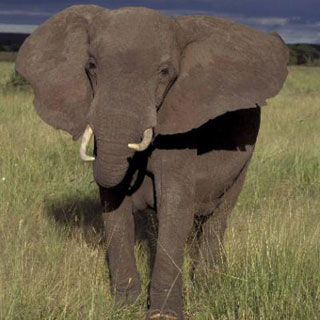
\includegraphics[width=0.8\linewidth]{elephant.jpg}
        % Example of an in-line image
    \end{center}

    Integer id congue eros. Phasellus venenatis pulvinar nisl, sed ultrices arcu
    vulputate non. Mauris at congue arcu, eget sollicitudin purus. Phasellus
    ullamcorper erat sed leo molestie, non ultrices enim aliquam. Donec cursus,
    arcu vitae ultricies euismod, massa ante ornare nunc, et porttitor erat augue
    iaculis nisl. Mauris ornare neque nisl, non pretium dolor adipiscing nec. Nulla
    nibh est, aliquam sed sollicitudin vel, imperdiet ut ante.

    %-----------------------------------------------------------

    \NewsItem{The fifth news item}
    \NewsAuthor{Author Name}

    Donec non nisl a arcu consequat varius. Sed suscipit cursus luctus. Nulla sit
    amet elit augue. Curabitur scelerisque mollis dolor, quis blandit lorem
    condimentum at. Pellentesque sed nibh vel dolor sagittis semper. Maecenas lacus
    enim, suscipit ut suscipit eget, feugiat vitae elit. Sed volutpat justo nisi,
    ac bibendum ante. Sed lacinia eros in massa euismod a iaculis metus fringilla.
    Integer dapibus nulla id purus consectetur. Pellentesque sed nibh vel dolor
    sagittis semper. Fusce placerat ultricies massa sed tristique. Aenean mattis
    nulla id eros adipiscing, vel pulvinar augue vehicula.

    \begin{quotation} % Example of a quotation
        \noindent{\Huge``}

        \noindent\normalsize\textit{Donec non nisl a arcu consequat varius. Sed
            suscipit cursus luctus. Nulla sit amet elit augue. Curabitur scelerisque mollis
            dolor, quis blandit lorem condimentum at.}

        \hfill{\Huge''}

        \hfill-- John Smith
    \end{quotation}

    Fusce placerat ultricies massa sed tristique. Aenean mattis nulla id eros
    adipiscing, vel pulvinar augue vehicula. Cras ultricies non turpis sit amet
    tincidunt. Quisque mollis vitae felis eu feugiat. Sed nec vehicula dolor. Nulla
    egestas vehicula nisl sed vehicula. Etiam ipsum dolor, aliquam eget sapien
    mollis, tempus elementum mi. Vivamus a auctor sem. In fringilla nunc at
    imperdiet rhoncus. Integer sagittis iaculis libero, at ultricies neque laoreet
    ac.

    \begin{center}
        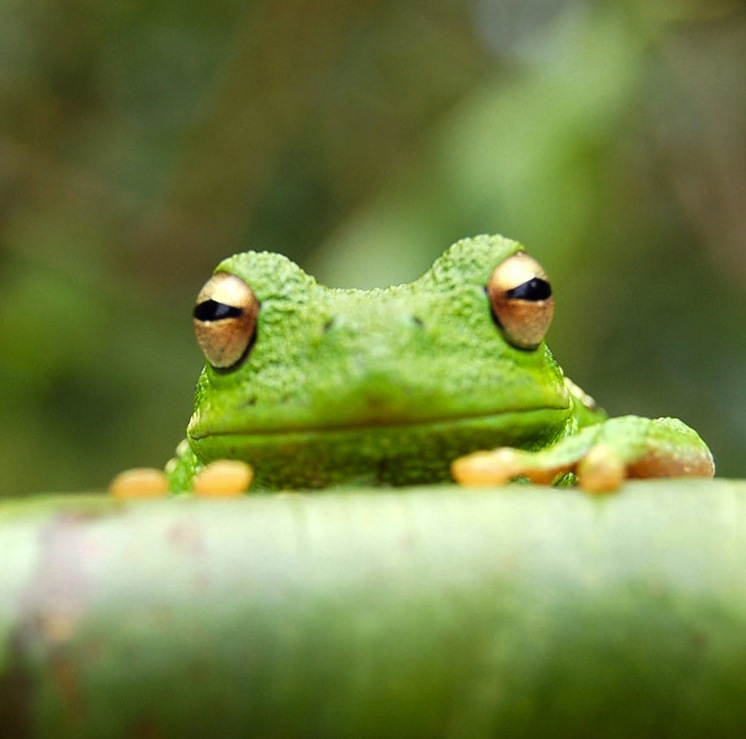
\includegraphics[width=0.8\linewidth]{frog.jpg}
        % Example of an in-line image
    \end{center}

    Integer id congue eros. Phasellus venenatis pulvinar nisl, sed ultrices arcu
    vulputate non. Mauris at congue arcu, eget sollicitudin purus. Phasellus
    ullamcorper erat sed leo molestie, non ultrices enim aliquam. Donec cursus,
    arcu vitae ultricies euismod, massa ante ornare nunc, et porttitor erat augue
    iaculis nisl. Mauris ornare neque nisl, non pretium dolor adipiscing nec. Nulla
    nibh est, aliquam sed sollicitudin vel, imperdiet ut ante.

\end{multicols}

%----------------------------------------------------------------------------------------

\end{document}